\documentclass[11pt,letter]{article}
\usepackage[top=1.00in, bottom=1.0in, left=1.1in, right=1.1in]{geometry}
\renewcommand{\baselinestretch}{1.1}
\usepackage{graphicx}
\usepackage{natbib}
\usepackage{gensymb}
\usepackage{amsmath}
\usepackage{lineno}


\def\labelitemi{--}
\parindent=0pt

\begin{document}
\bibliographystyle{/Users/Lizzie/Documents/EndnoteRelated/Bibtex/styles/besjournals}
\renewcommand{\refname}{\CHead{}}
\begin{flushright}
Version dated: \today
\end{flushright}
\bigskip
\noindent RH: Interactive cues and spring phenology
% put in your own RH (running head)

\bigskip
\medskip
\begin{center}

% Insert your title:
\noindent{\Large {\bf Concept paper on understanding interactive cues and climate change (with growth chamber studies)}}\\
\vspace{2ex}
{\Large (1) How interactive cues will shape climate change responses \\
\vspace{2ex}
(2) Limiting cues: How spring warming, winter chilling and daylength will shape climate change responses}\\ % Ailene likes 2 best
\vspace{2ex}
% (3) Spring warming, winter warming or daylength: What cue will be most limiting in future tree phenology?} % What cue will be most limiting with climate change? Forcing x photoperiod x chilling
% Isabelle likes 3 best, but Lizzie feels it is not the topic of the paper.
\bigskip

\noindent {\normalsize \sc
The lab in 2017$^{1,2}$}\\ % Ailene, Cat, Dan, Lizzie, Nacho
\noindent {\small \it
$^1$ Arnold Arboretum of Harvard University, 1300 Centre Street, Boston, Massachusetts, 02131, USA\\
$^2$ Organismic \& Evolutionary Biology, Harvard University, 26 Oxford Street, Cambridge, Massachusetts, 02138, USA\\
$^3$ Forest \& Conservation Sciences, Faculty of Forestry, University of British Columbia, 2424 Main Mall, Vancouver, BC V6T 1Z4}\\

\end{center}
\medskip
\noindent{\bf Corresponding author:} Lizzie, see $^{1,2}$ above ; E-mail:.\\

\newpage
%\linenumbers

\begin{abstract}
Climate change has shifted plant phenology globally, with average shifts of 4-6 days per $\degree$ C and some species shifting much more. Globally, such shifts have been some of the most reported and most predictable biological impacts of climate change. This predictability comes from decades of research, which have outlined the major cues that drive most studied plant phenology: temperatures (including spring warming and winter chilling) and daylength. Further simplifying predictions, spring temperatures are often the dominant cue in nature, making linear models of heat sums often excellent at predicting interannual variation in phenology. Yet as climate change has marched on, new research has uncovered possible failures to predict the current observed changes; increasingly, phenological shifts appear more muted over recent decades, or in certain locations. Here we argue that some of these inaccurate predictions are due to simple models that neglect to consider other major cues---especially winter chilling and daylength, which moderate and shape plant phenological responses to spring warming. We highlight how over 60 years of research in controlled environments can improve predictions for when, where and how the interactive effects of other cues will impact simple linear predictions. Finally, we discuss how a new generation of controlled environment experiments could rapidly improve our predictive capacity for woody plant phenology in coming decades.  % Change tone here to -- we need better understanding of these other cues if we want to understand shifts across space and time. 
\end{abstract}

\noindent \emph{Main message (and, really, it's important):} If you want to project climate change impacts, you need to focus on relevant changes in all three cues. The relevant changes part is about comparing cues, the all three cues is about interactive cues.

\noindent \emph{Keywords:} phenology, climate change, spring warming, chilling, forcing, daylength, photoperiod, non-linear responses, leafout, budburst\\

\newpage
\linenumbers
\section{Main text}
Shifts in spring plant phenology are one of the most reported and most predictable changes with climate change. Decades of research have documented advancing budburst, leafout and flowering across systems \citep{delpierre2009, yu2010,Ellwood2012,jochner2013,hereford2017}, especially in temperate systems where long-term records make a strong case for how humans have altered the timing of spring \citep{Schwartz:1997nn,Menzel2003a,Menzel:2006}. Recently, however, these advances have appeared to slow \citep{fu2015} or even reverse in some places \citep{yu2010}---failing to match simple predictions of an advancing spring with continued warming \citep{Ellwood2012}. The main hypothesis for this failure is that spring warming---which most observational studies focus on---is no longer the only cue that matters to predicting responses to continued warming \citep{chuine2016,gauzere2019}.\\

Despite the focus of much spring phenology research on spring warming, increasing evidence suggests the underlying physiology of spring phenology is more complicated for most temperate species (ADDCITES). For many species three major cues drive spring phenology: forcing (warm temperatues, generally occurring in the late winter and early spring), chilling (cool temperatures, generally occurring in the fall and winter), photoperiod (daylength). Forcing and chilling cues are generally understood to be accumulation processes, where plants must integrate chilling and forcing experienced over time to meet a sum threshold value at which they can budburst, leafout or flower \citep{Chuine2000}. In contrast, photoperiod is generally not considered an integral cue, but one evaluated daily \citep{Singh:2017}. \\

Together, forcing, chilling and photoperiod cues may produce non-linear responses that many current methods do not predict \citep[e.g.,][]{Ellwood2012}. Predicting these non-linearities is a common goal in plant phenology research today \citep{gusewell2017, martlusch2017,gauzere2019,chen2019,keenan2019}, but has been slowed by data gaps and the underlying complexity of spring phenology. \\

The first step towards improved phenological predictions is robust measurements of chilling, forcing and photoperiod cues. Recently, much effort has focused on estimating these cues from long-term observational data. Yet observational data may often fail to robustly estimate any of the three major cues due to two types of statistical issues. First, in most observational data these cues are correlated: forcing increases alongside longer days (CITEAILENESARAH), and chilling and photoperiod cues both yield similar predictions (i.e., both cues predict later spring phenology with warming). Second, most observational studies focus on linear models of each cue and often without interactions between cues. \\

Using simple linear models with observational data may make sense as phenological responses to most cues are expected to be linear except at extremes. Natural conditions often see only a small slice of the range of values of each cue that are possible---and those values often appear to be in the middle linear range (CITES). Further, given that interactions between cues are difficult to estimate---more-so when those cues are highly correlated in nature---focusing on main effects of cues that integrate over any interactions (CITES) may provide the more robust estimates from oberservational data.  In contrast to the limitations of observational studies, one method is designed to robustly measure the complexcity of cues: controlled environment (e.g., growth chamber) studies \citep{nagano2012,satake2013}.\\

Controlled environment studies of plant phenology have been conducted for over 70 years and are specifically designed to understand non-linearities both in individual cues and produced by interactions between cues. In contrast to observational studies, controlled environment studies can manipulate all three cues, extend to other cues that may be important in some species or biomes (e.g., humidity, drought conditions, light spectra), and can tease out interactions between cues by experimentally decoupling them. Despite the prevalence of growth chamber studies for spring phenological cues, they have rarely been reviewed. Perhaps more surprisingly, they have been often poorly integrated into the current phenological literature on climate change. This includes in debates where they are critical---such as about the importance of photoperiod \citep[e.g.,]{fu2015,richspurce2018}.\\

Here we aim to help integrate the long-term literature on growth chamber studies into current phenological research on climate change more fully. We begin by outlining how the three major phenological cues---forcing, chilling and photoperiod---can produce non-linearities and how they will shift in coming decades with anthropogenic climate change. We then review 70 years of controlled environment studies to understand how much of the cue-space (possible natural range of each cue and interactions across cues) has been studied and how experimental treatments compare to shifts in cues caused by climate change. Based on this, we discuss how controlled environment studies can be best designed to understand interactive cues and build more robust predictions.\\ 

Given our aim to improve understanding of current trends and forecasts we focus on early vegetative phases (budburst and leafout) of wild species, which are critical to plant growth and thus to models of carbon uptake and storage, and which have shifted most with climate change \citep{Cleland:2007or,IPCC:2014sm}. We touch on other areas of research, which have been important to our understanding of the cues underlying phenology. In particular, research has been especially strong in model systems (e.g., \emph{Arabidopsis, Populus}) and crops \citep{cesaraccio2004}---with the exact phenophase of interest varying (potentially by a species' life history: more focus on germination and flowering in \emph{Arabidopsis}, and more on leafout and budset in \emph{Populus}).  Given our focus on budburst and leafout, our review concentrates on woody species phenology, where most research has been conducted. Most of our conclusions and suggested approaches, however, could be adapted to apply to non-woody species and/or other phenophases with similar underlying interactive cues. \\

\subsection{How do phenological cues produce non-linear responses?}
The major phenological cues of forcing, chilling and photoperiod can produce non-linear responses through each cue alone when examined across a sufficently wide range of values. Cues may be linear in the mid-range of values, while extremely high or low values of some cues may produce alternative response \citep{gauzere2017}. For example, at very low photoperiod (short days) plants often will not grow or budburst erratically (CITES), similarly maximum growth may occur at photoperiods of 18 hours, meaning photoperiods longer than 18 hours will have no additional effect on budburst timing \citep{major1980}. Similarly, extrememly cool or very hot temperatures may limit forcing as plant developmental processes slow (CITES). Such extreme values of cues, however, are likely less common than interactions between cues that can produce non-linearities.\\

Forcing, chilling and photoperiod cues together generally determine budburst each year in many temperate species, with the amount of forcing needed determined by the level of chilling over the fall and winter and by the photoperiod while forcing is accumuulating in the spring. Higher forcing is generally needed given lower chilling (see FIGURE) and short photoperiods (CITES)---producing generally a subadditive effect of forcing x chilling and forcing x photoperiod (i.e., both cues together produce a more muted response than the addition of each cue's effect alone). This interaction of cues produces a non-linearity in environments where levels of cues are correlated over time or space; for example if chilling declines are correlated with greater forcing, and may be critical to accurate forecasts with climate change. \\ % The interaction of interactive cues with common environmental correlations may cause additional non-linear complexities (e.g., warm springs may cause mean plants meeting their forcing cues at shorter photoperiods). 

The complexity of cues for spring phenology likely allows species to maintain their fitness across relevant spatiotemporal environmental variation CITES. In the spring, selection for species to track the start of resources each year (to gain access to them before other individuals have depleted them) without major tissue loss to frost, herbivores or other factors (CITEs) should select for cues that work across the interannual variation in climate across of their ranges. Species thus need cues with either plasticity and/or local adaptation. Spring phenology can be fairly plastic \citep{vitasselev,kramer2017}. Especially compared to other phenophases, such as budset phenology, budburst and leafout often do not show high local adaptation across a range \citep{mimura2010}. This means that species ideally need a set of cues that work across their range \citep{liepe2016}, though there may be variation in the importance of each cue across a range \citep[e.g., chilling can be higher in coastal versus continental, see][]{campbell1979}, and genetic work suggests the same genes can be triggered by very different environmental cues \citep[e.g.,][]{simpson2002arab,Stinchcombe:2004ec}. \\

% FIX ME! Fix section on non-linearities from intxns... Also, add schematic figure here? Nacho writes could we give examples of non-linearities at the extremes? (e.g. thresholds, asymptotical, saturating, negative exponential, etc.)
These cues may create non-linear responses with warming in two major ways. First, as discussed above, each cue non-linear ... Secondly, interactions between cues

\subsection{How will chilling, forcing and photoperiod shift with climate change?}
Indeed, one of the most critical changes that can happen is when pre-climate change conditions generally caused budburst to occur at the extremes of some cues (e.g., high chilling and/or long photoperiods, where responses may be effectively muted) and climate change has now pushed budburst into periods where these cues are at the more linear part.\\ 


All three cues are expected to shift with climate change (See Fig. \ref{fig:pep}), though the shifts will vary substantially across space and time. Most notably to date, warming increases the forcing plants experience each day, with more rapid shifts---and thus also greater shifts---at higher elevations and in the arctic \citep{IPCC:2014sm}. Daily minima (generally night-time temperature) will generally warm more than maxima temperatures, though this effect varies spatially \citep{Alexander:2006qy}. Warming across seasons is also variable \citep{Alexander:2006qy}. \\ % Cat writes: Important stuff here but I think we need to add some more information: Why are shifts in daily minima temperatures so important versus maxima temperatures? ’…though this effect varies spatially’, is this more common at higher elevations and in the arctic? Or elsewhere? ... I like where you’re going with the last sentence as a transition into chilling but maybe we can say more here? Maybe something like “Warming across seasons is variable with warming not only influencing forcing temperatures in the spring, but it is also contributing to shifts in chilling in the winter.” ... Dan also said this last bit was confusing and said more clearly below ("These cues may create non-linear responses with warming in two major ways.").

Warming also translates into important shifts in chilling, though our poor understanding of chilling makes predicted shifts in chilling complicated \citep{chuine2016}. Research to date suggests chilling only accumulates in a certain range of temperatures with low (e.g., $<$0$\degree$C) temperatures generally not contributing to chilling accumulations and higher temperatures (e.g., $>$12$\degree$C) potentially decreasing previously accumulated chilling \citep{richardson1974,fishman1987}. Thus, major shifts in accumulated chilling would be predicted where temperature regimes that were previously too low to accumulate chilling in many months of the winter warm such that chilling now accumulates in those months \citep{guy2014}. Areas with this shift would then expect much earlier budburst with warming, potentially far earlier than last frost dates. 


% Cat writes: I think we might want to move these lines somewhere else… since this section is focusing on the effects of climate change on cues, I feel these lines—though important—are distracting from the main message of this section 
Unfortunately, these predictions are based on models developed almost solely for agricultural crops \citep[but see][]{harrington2015}, especially stone fruits, and have rarely been robustly adapted to forest trees. While the development of classic models of chilling for peaches and related fruit trees benefited from data on these species being planted far outside their range into regions with extremely low or potentially no chilling, equivalent data on forest trees is almost never available \citep{dennis2003}. Thus chilling models to date generally use limited observational and experimental data from forest trees to try to reparametrize the basic stone fruit models \citep{Chuine2000}.\\

Improved chilling models for forest trees (and horticultural trees) may come from an improved understanding of dormancy at the physiological level. Chilling is defined as what leads to break of endodormancy, after which plants enter ecodormancy when accumulated forcing then leads to budburst \citep{chuine2016}. Measuring endodormancy and its transition into ecodormancy is notoriously difficult, however, and work to date has relied generally on cellular staining methods tested on a very limited subset of species \citep{rinne2011}. These methods themselves rely on a still-developing understanding of what causes dormancy at the cellular level \citep{vanderschoot2014}. In practice, most phenology studies use the terms `chilling' and `forcing' to mean `cool temperatures' (often either in the fall and winter or applied in experimental conditions) and `warm temperatures' (often either in the spring or applied after sufficient chilling) and generally hope they correspond to endo- and eco-dormancy. Some studies use the sequential transfer of cuttings to warm conditions to estimate the transition from endo- to eco-dormancy, with rapid and full (e.g., $>$90\% of buds on a cutting) budburst generally meaning a plant is ecodormant \citep[e.g.,][]{Junttila:2012aa}, but given that this is labor- and space-intensive most studies considering chilling do not do this. We expect that without a much improved physiological understanding of endodormancy release robust models of chilling---and thus accurate predictions of how chilling will shift with climate change---will be difficult to develop. \\ % And there is so much we don't know about how chilling works and interacts with forcing (sequential model, parallel models etc.)
% Nacho sayd: could we say this in a positive note? i.e. what should be done to make more robust models? 
% End of Cat's concerns

% Need better transition here.
Research has addressed shifts in photoperiod with climate change far less often compared to predicted changes in forcing and chilling \citep[but see][]{saikkonen2012,way2015}. While an environment's photoperiod does not shift with climate change, the relevant photoperiod a plant experiences at critical physiological points may change dramatically with warming. In particular, increases in chilling and/or forcing, which could alone produce much earlier budburst, may be offset by short photoperiods that delay budburst \citep{gauzere2019}. Similarly, long photoperiods can lead to budburst sooner than predicted by solely low chilling or forcing conditions \citep{Nienstaedt:1966aa,Myking:1995,Partanen:1998aa}. Thus, changes in chilling and/or forcing correspond to changes in the relevant photoperiod with climate change. \\


% Ailene notes: these conditions are what we need a schematic figure for, i think, as it is referenced throughout the manuscript.
% Nacho writes: This paragraph is a bit hard to follow, perhaps sticking a bit more to Fig 2 (by linking the examples to it) would help?
Given our current understanding of phenological cues, we should expect the most dramatic changes in phenology in systems with non-linear responses where climate change pushes the system across a critical threshold or inflection point. For example, if some species have a critical photoperiod for budburst and warming means forcing cues are met before the critical threshold, then we would expect incomplete or highly delayed budburst (needCITES). Similarly the complexity of chilling could produce myriad non-linearities. If, as currently hypothesized, chilling follows an optimum curve (i.e., chilling does not accumulate at very low or high temperatures but in between it accumulates at a maximum rate at some temperature optimum), then endodormancy break would shift earlier in systems where warming pushes winter temperatures into a chilling-accumulation temperature or closer to the optimum temperature, and delay where warming pushes winter temperatures beyond the optimum (with more complex predictions if high temperatures decrease accumulated chilling). Interactive cues could also produce non-linear responses, but predicting these requires a refined understanding of the interaction and whether there are critical inflection points that may be crossed with continued warming. These complexities highlight how difficult predictions may be without careful efforts to tease out how each cue works alone and interactively. 

\subsection{Predicting non-linear responses with controlled environment experiments} % or just forecasting future responses?

% Nacho writes (middle of below paragraph): and if enough treatments allow fitting such complex models, right? Maybe that is what is meant by a relevant range, but I would emphasize that even within the relevant range, if you only have two-three treatments per cue, that may capture interactions but not be enougth to forecasts non-linear responses.
Controlled environment (generally growth chamber) studies can help predict non-linear responses by allowing researchers to examine the effects of one cue with the others held constant, and examine interactive effects, given the appropriate study design. Such experiments may be especially useful for forecasting if they are designed in a range relevant to current versus future conditions. Indeed, one of the major advantages of experiments is that they allow treatments outside of the historical range---an option long-term observational data can never provide. We reviewed controlled environment studies over the last seven decades (1947-2014) to understand the range of treatments already available, and how they compare to current and future conditions. We note that these studies were rarely conducted for climate change research, and most often done for fundamental science or other areas of applied science (e.g., horticulture or forestry). Yet they are some of the best available data for how plants respond to the environment and thus a critical resource for climate change research today.\\

Controlled environment studies have been conducted across 227 species across the globe, with the majority of papers report research occurring in Europe (54 of 85 papers), followed by North America (23, Fig. \ref{fig:datamap}). Most studies manipulate one cue (Fig. \ref{fig:ts}), though studies of two or three cues have occurred in almost every decade. Forcing and photoperiod were the most commonly studied cues (56\% manipulated forcing; 55\% manipulated photoperiod), with chilling being studied in only a third of all studies (33\% manipulated chilling). The actual cues studied varied across latitude with a general trend toward examining more extreme values at higher latitudes. Thus, forcing and chilling treatments decline 0.1$\degree$C per 1$\degree$ latitude (for forcing, min is -0.12, for max it's -0.08, see Fig \ref{fig:lat}; for chilling it's -0.1 for min and -0.07 for max); and the maximum studied photoperiod increases with latitude (0.08 hr per degree $\degree$ latitude). These shifts across space appear related to differences in extremes across latitudes (higher latitudes experience colder temperatures and longer photoperiods), but introduce a bias in results as any comparisons of studies from lower and higher latitudes are also comparing a different range of cues generally. \\
% See countintxns.R 
% Need to add: 
% (1) Table of all analyses to supp
% (2) Say something about material (seeds/saplings/cuttings)? Can we tie to relevance of predicting future forest communities or such?

% Dan found this paragraph hard, consider adding sub-heading and maybe this structure:
%  OSPREE studies can be broadly categorizes into these type of studies 
% Studies that manipulate 1 cue: Paragraph about them
% Studies that manipulate 2 cues: Most test photo and forcing\\ Weiburger
% Studies that test all three: Very rare
% This also might highlight the rarity of full interactive studies and help drive home why our predictions may suffer for it.
Single cue studies were the most common, but prevent understanding interactions among cues or comparisons of which cues dominate phenological responses; studies of multiple cues can overcome these challenges. Of the studies manipulating at least one cue, half additionally manipulated another cue. Study designs most often allowed examining whether cues were interactive (that is, whether the effect of one cue depends on the level of the other cue), with the most studies testing for interactions between photoperiod and forcing (21 studies), followed by studies that examined the effects of photoperiod (13 studies) and forcing (12 studies) across the fall-winter. Such studies follow the design generally attributed to \citet{weinberger1950} where tissue (e.g., cuttings) are taken progressively across the fall and/or winter seasons then exposed to controlled environment conditions. These studies often equate tissue removed later from the field as having received more chilling and thus often treat `time of cutting' as interchangeable with `chilling,' though forcing and photoperiod conditions also change. Studies examining photoperiod or forcing crossed with experimental chilling treatments (either through changes in temperature or days of chilling) were much less common (8 studies each for photoperiod and forcing). Studies examining three cues directly were very rare: we identified only two studies examining all three cues at once, and both were on \emph{Picea abies} \citep{Worrall:1967aa,Sogaard:2008aa}. A slightly larger set of studies (5 studies) examined three cues indirectly---manipulating photoperiod and forcing in controlled environments but equating chilling with sequential removal of tissue from the field---for 11 species \citep{Schnabel:1987aa,Heide:1993,Partanen:1998aa,Basler:2014aa}. \\
% I think we need to add what the interactive studies found -- did they all find interactions? 
% "okie11_exp2"  -- Peach, doesn't really cross forcing (mainly chill x photo)   "worrall67_exp 3" (this paper coolly opens with "As has been repeatedly emphasized in the literature, discussions of dormancy in woody plants are often misleading because of the lack of a standard nomenclature.") and "sogaard08_exp2" .... both on Picea abies
% "basler14_exp1" (Acer pseudoplatanus. Fagus sylvatica, Quercus petraea, Picea abies)  "heide93_exp1"    "heide93_exp2" (heide93 was Alnus incana, Alnus glutinosa, Populus tremula, Prunus padus, Betula pubescens, Betula pendula)  "partanen98_exp1" (Picea abies) "schnabel87_exp1" (Vitis vinifera) -- all checked

The paucity of studies examining multiple cues limits our fundamental understanding of each cue, as well as how---when combined---they will determine future leafout with continued warming. Because the cues are all known to be interactive, estimates of any one cue are influenced by the level of each other cue. Knowing the level of each other cue is difficult both because they are often not reported, and also because they are somewhat impossible to know given our current understanding of endodormancy (when we understand chilling is accumulated) and ecodormancy (when we understand forcing is accumulated). Authors may use the terms `chilling' and `forcing' for their treatments, but they rarely have physiological evidence that these are the actual conditions plants experience. Studies using sequential removal from the field to estimate chilling are at perhaps the greatest disadvantage to estimate the cues applied: chilling must rely on field estimates from models that are currently only hypotheses of actual chilling \citep{dennis2003}, and forcing and photoperiod treatments are most probably a mix conditions in the field and conditions applied in controlled environments. \\% Further any study conducted over much of the fall and winter is most likely estimating the effect of their `forcing' and photoperiod treatments on first endodormant plants, and then ecodormant plants---with when the switch happened generally unknown. Some studies do attempt to assess dormancy state ... [we need to add more here!]. [... end on needing more studies of interactive cues or just more studies reporting dormancy state and best guess at other cues?] 

The utility of controlled environment studies to forecasting also depends on how relevant treatments are to current and future conditions. Estimating such relevance is difficult as it depends on a species' range and projections considered. However, a, simple analysis of two widely studied species, \emph{Fagus sylvatica} and \emph{Betula pendula}, suggests experiments have generally bracketed the range of projected temperatures. Projected changes in maximum temperatures generally fit within the range of temperature differences conducted within forcing treatments in experiments (e.g., an experiment with both 16$\degree$C  and 20$\degree$C forcing treatments would have a 4$\degree$C difference), and similarly matched differences in minimum temperatures in chilling treatments. As we noted above, however, there is a paucity of chilling studies that directly manipulate chilling temperature---and thus allow a comparison of how differences in chilling temperatures impact phenology. Indeed, we found no studies with multiple chill temperatures tested for \emph{Fagus sylvatica}, even though it is one of the most well-studied species. \\

% While experimental shifts included the range of climate projected temperature change... 
Experimental shifts were generally larger than expected shifts due to climate change. This makes sense from an experimental-statistical perspective: if the goal of an experiment is to identify if a cue is present then larger treatment differences should yield larger effect sizes and thus higher statistical power. But such large shifts may be risky to extrapolate to smaller shifts due to warming. Further, experimental studies vary from natural settings in myriad ways. Different studies have ameliorated some of these differences. For example, most studies (34 of the 48 that manipulated forcing) have constant day/night temperatures, but some vary day and night temperatures (26) with nights generally being cooler, while some have even introduced ramped temperature through the day and across an experiment's length \citep[e.g.,][]{Basler:2012,Laube:2014a}. Yet these shifts are generally introduced in experiments that are not designed to test the effect of a controlled environment more similar to natural conditions \citep[but see][]{erwin1995} and thus provide little insight on how much such experimental artifacts matter. % Fix this previous sentence, it's confusing
Such differences mean extrapolating from controlled environment studies should be done with care, and highlight a need for future experiments designed to improve forecasting effects of climate change. 

\subsection{Paths forward} % Nacho writes: I love this section, can use a bit of polishing, but makes the paper more exciting and relevant. (Yay, says Lizzie)
We argue that controlled environment experiments will be critical for accurate predictions of phenology given future warming, How accurate such predictions are will depend on the design of future experiments and how well they can be integrated with long-term data to improve models. % START HERE and put in the rest of the comments

\emph{Improving controlled environment studies}\\
We expect the most useful future experiments will be designed to improve models. In particular, experiments designed to identify threshold effects and optimal temperatures/photoperiods, and non-linearities from interactive cues may be most useful. Identifying threshold effects and optimal temperatures or photoperiods generally requires many different levels of a single cue, which can make such experiments difficult to cross with other cues. Yet, understanding if findings are consistent across varying levels of other cues should be a follow-up step to confirm that findings can be applied across levels of other cues. Studies manipulating more than one cue also test for non-linearities due to interactive cues, as long as they are fully-crossed (i.e., every combination of levels is present in treatments; for example, a study with two photoperiod and three forcing levels would need six different treatments). Such experiments can quickly require a large number of controlled environments, but provide critical information for models and to connect to long-term findings. As growing experimental results support that all cues are dependent on the level of other cues \citep{stearns1958,flynn2018} and long-term data hint at multiple cues \citep{fu2015}, we believe this should be a major research aim.\\

Controlled environment studies may also be more readily applied to forecasting by exploring more realistic conditions. While identifying thresholds, optima and non-linearities may involve considering informative extremes in levels of cues, most changes in cues due to climate change are on a (relatively) smaller scale (Fig. \ref{fig:pep}). Thus, when designing studies to contribute to improved forecasting of particular species, experimentalists should examine cues within the current and projected future range of species. In most species distribution models, species are expected to remain in the same climatic conditions, suggesting there may be minimal changes---assuming such models of species distribution are accurate and that species track perfectly. [Alt: Most species distribution models assume that species occupy a consistent climate envelope with climate change; that is, species will track current climate conditions by moving in space.] Most evidence, however, suggests species will lag in their spatial responses \citep{Loarie:2009ax}, meaning shifts in cues in the current range may be important to the fate of trailing edge populations \citep{bertrand2011changes,lenoir2015climate,savage2015elevational}. Beyond the absolute level of cues, controlled environment studies need more work on what attributes of the design are more or less critical for replicating responses from the field. For example, controlled environment studies have shown differing day/night temperatures are important for some species \citep{heuvelink1989influence,abrol1996effects,Thingnaes2003,pressman2006exposing}, but comparison studies have not been conducted for most species. Equally, a few studies have attempted to replicate certain aspects of the environment, such as fluctuating temperatures, ramped temperatures and light throughout the day, the coincidence of temperature and sunrise \citep{erwin1998}, but these are by no means widespread enough to understand how important these conditions are for extrapolation to models. \\

\emph{Improving integration of controlled environment studies with long-term data}\\
% Nacho writes: I guess we don't want to go there, as it would complicate things even further but it would be great if experimental designs included measuring physiological responses to see how strongly connected they are to the phenological ones.
A major need currently is improved integration between long-term data and controlled environment studies. With important exceptions \citep{gauzere2017}, studies of long-term observational phenology data have moved forward independently from controlled environment studies. Recent observations of declining responses to warming in long-term data suggest cues beyond forcing may be playing a role \citep{fu2015} and highlight the major need for non-linear models based on interactive cues. To this aim, a number of recent papers have attempted to identify chilling or photoperiod cues in long-term data. Correlations between these predictors, however, are almost always too high for any useful analysis (needCITES). Other approaches that attempt to break some of these correlations, such as leveraging elevational or latitudinal gradients, may run afoul of other correlations---for example, gradients in local adaptation that mean cues shifts along these gradients in complex ways \citep{tansey2017}. Similarly, controlled environment studies, as we have reviewed here, generally do not use long-term data to help interpret results or define treatments. \\
% Should we add a figure here? Since budburst reviewer 1 did not believe us... (maybe look at some of the papers and pull data) or use what Dan B. has already done?

While most studies of long-term data and controlled environments generally ignore one another, attempts to integrate the two provide a useful path forward \citep{Caffarra:2011qf,nagano2012,satake2013,ford2016,chuinearees}. Experiments that test for thresholds and the presence of important interactions have helped re-design models \citep{Caffarra:2011qf,chuinearees}, while other studies have used experiments to test extremes (e.g., extremely low chilling) combined with data from long-term provenance studies to understand how growth and phenology will combine to determine future ranges \citep{ford2016}. Further, some work has used controlled environments to test model predictions, especially in future climate scenarios where non-linearities are predicted \citep[see][]{nagano2012}. Such work underlies progress towards model development that relies continuously on a back-and-forth process between developing models based on both long-term data and experiments, then testing predictions with new experiments and as newer observational data are generated (i.e., more years and also data from new locations) \citep{nagano2012,satake2013}. Such efforts of continual development take extensive data and thus have only been carried out for a very few species [add species and cites].\\
% Caffarra:2011q: betpen
% nagano2012: rice plants
% satake2013: Arabidopsis halleri
% ford2016: Doug fir

\emph{Building species-rich predictions}\\
Given the efforts and data involved in models for a single species, building up to multi-species predictions may appear daunting, but multi-species models are crucial for accurate forecasts that can apply to diverse regions and large-scale vegetation models. Addressing this issue requires, of course, more data. Long-term data is generally more species-rich than controlled environment studies. For example long-term observational data in the PEP725 and NECTAR databases together have multi-site data on more than 1,600 species, while our review of controlled environment studies found most studies focused on only one species with data on a total of 227 species. Thus, more diverse controlled environment studies may be the current major data limitation. Beyond data, however, new modeling approaches can help integrate current and future data more powerfully. \\

Bayesian hierarchical models are specifically designed for analysis of diverse datasets. With the right information and sufficient data, they can attribute variation across studies to the species studied, the cues (i.e., chilling, forcing and photoperiod levels in studies) and remaining unmeasured variation in studies (i.e., differences in chamber design may be captured by a `study ID' variable in such models). Such models are extremely powerful for building species-rich predictions as they leverage data across all species into one model designed to capture both the cross-species and cross-study overall effects as well as species-level differences. Yet, like all models, they are more robust with more data. In particular, attributing variation due to study versus species requires the same species to be studied across several studies, which is currently not the case for most species, according to our literature review (cite Table I need to build). Thus, these models will be most useful given greater efforts to publish data. Given proper data reporting (i.e., all cue conditions must be defined, even when not manipulated, and controlled environment conditions should be fully described including relative humidity and irradiance) all studies---whether designed to improve models or forecasting, or not---can be included in such models. 

\subsection{Right now: It's your tomorrow}
Research on phenology had been conducted for centuries before anthropogenic climate change caused earlier budburst and leafout across much of the globe \citep{Sparks:1995mv}. Decades of controlled environment studies contributed to our fundamental understanding of the drivers of spring plant phenology. Today, climate change requires leveraging these decades and centuries of research for more accurate predictions that can help humans adapt to warming. \\

We have outlined how researchers could better harness the power of controlled environment experiments to transform our fundamental understanding of phenology and advance forecasting. Controlled environment studies can critically rule out, or support, hypotheses to explain observed discrepancies in long-term data and open up new pathways to use long-term data to understand current trends, helping the field move beyond trying to tease out cues using only long-term data where cues are inherently correlated. While understanding, modeling and predicting interactions among cues and their effects on phenology is challenging, any advances would yield more accurate predictions, with valuable implications to more realistically assess the effects of climate change on plant biodiversity, including agricultural and forest species. 


\section{References}
\bibliography{..//..//refs/ospreebibplus}


\section{Figures}

\newpage
\begin{figure}[t!]
\centering
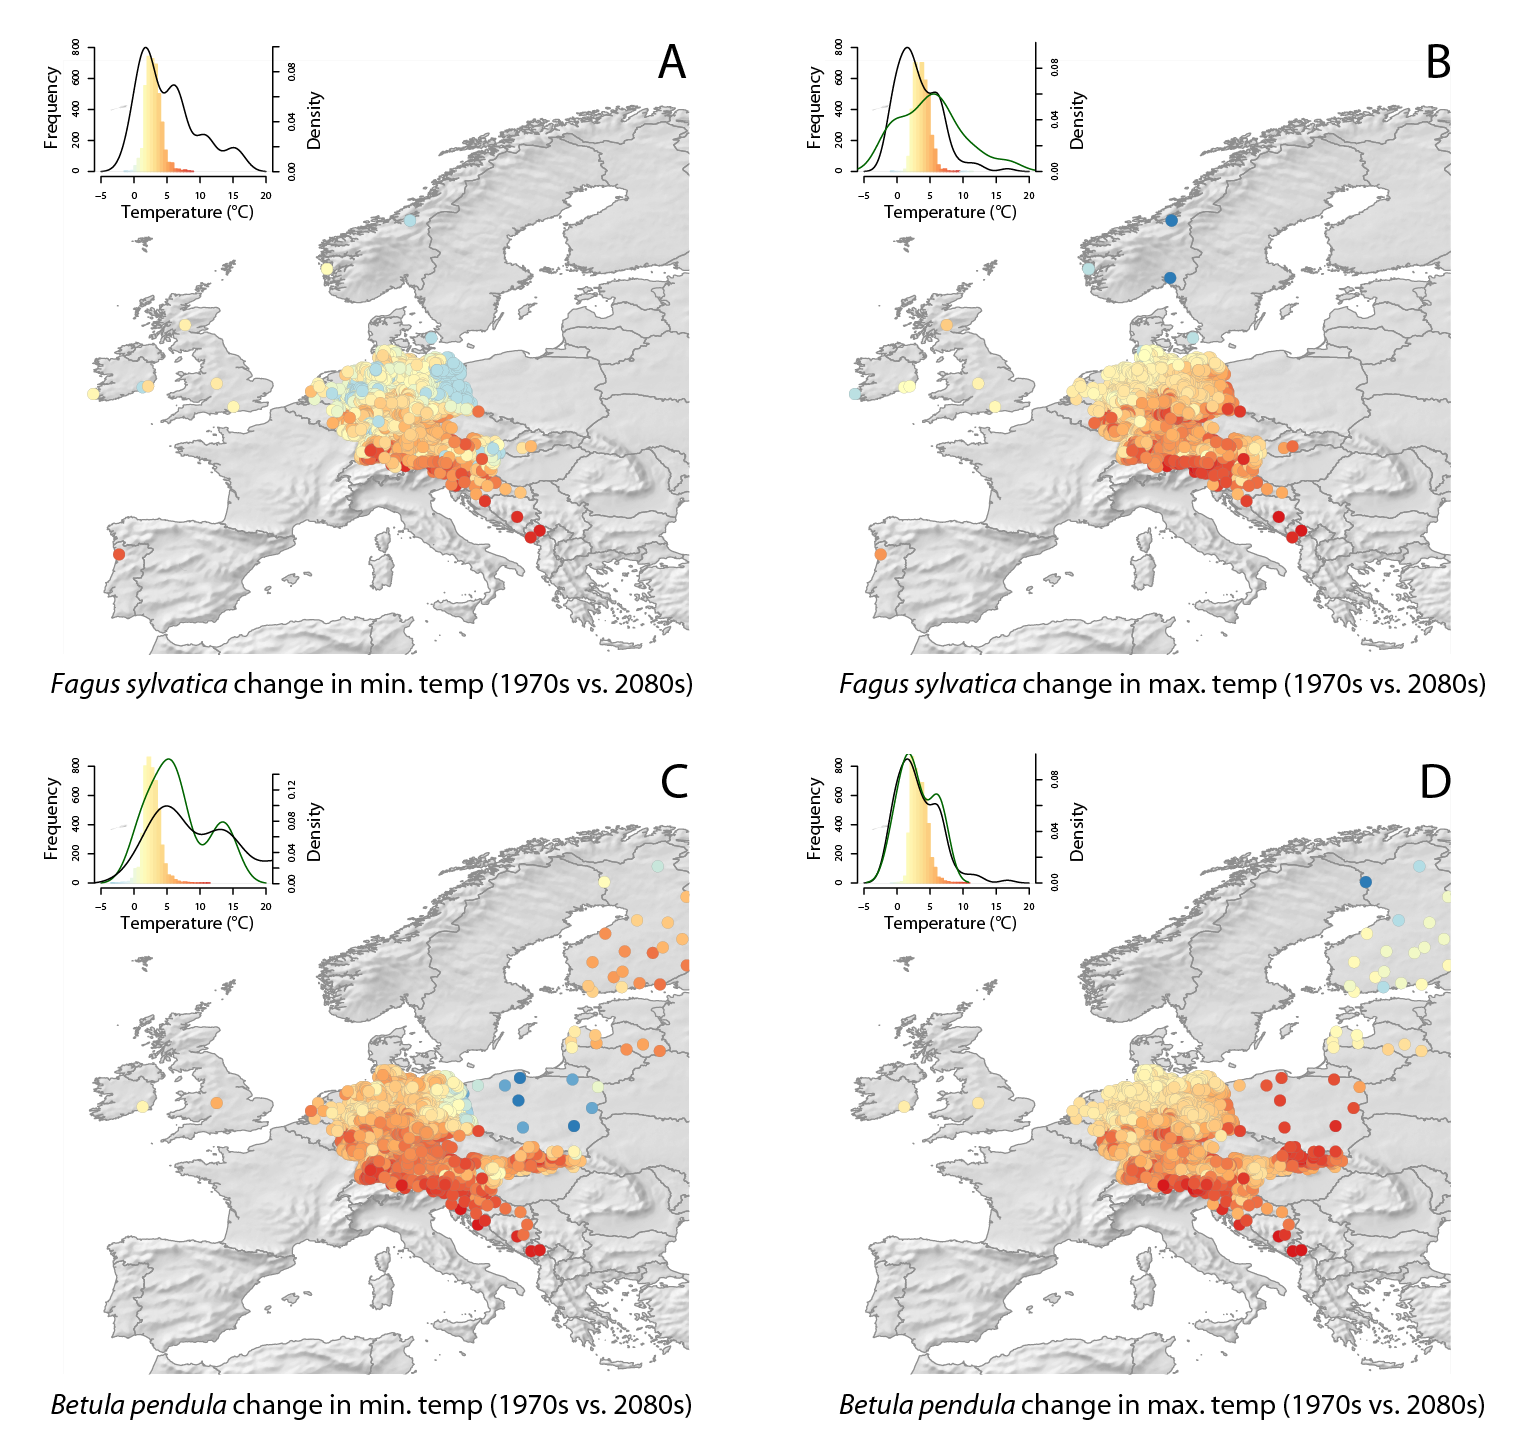
\includegraphics[width=1\textwidth]{figures/Fig1_noblues_densities.png}
\caption{Predicted changes in temperatures relevant to chilling (A, C) and forcing (B, D) compared to a 1970s baseline shown for two species: \emph{Fagus sylvatica} (A-B) and \emph{Betula pendula}. Points represent a PEP725 site with XX data. Inlay plots in the upper left-hand corner of each plot show a histogram of the predicted changes in temperature overlaid with densities of the chilling (A, C) and forcing (B, D) treatments (green lines show the treatments for that exact species, while black lines show across all species; note that for \emph{Fagus sylvatica} there are no chilling treatments of differing temperatures).} % Fix figure caption: This is a cool figure! I think the legend needs some additional detail to make it more clear. Specifically I would add 1) "...and forcing (B,D) treatments across XX studies;" 2) describe somehow that the color of the dots relates to the temperatures in the histogram. 3) It's not quite clear to me what "temperatures relevant to chilling...and forcing" are- does this mean winter temps vs spring temps? 4) Is the histogram showing changes in temperature or temperature? The axis label says temperature but the figure legend says changes in temperature. If it is temperature
  \label{fig:pep}
\end{figure}


\begin{figure}[t!]
\centering
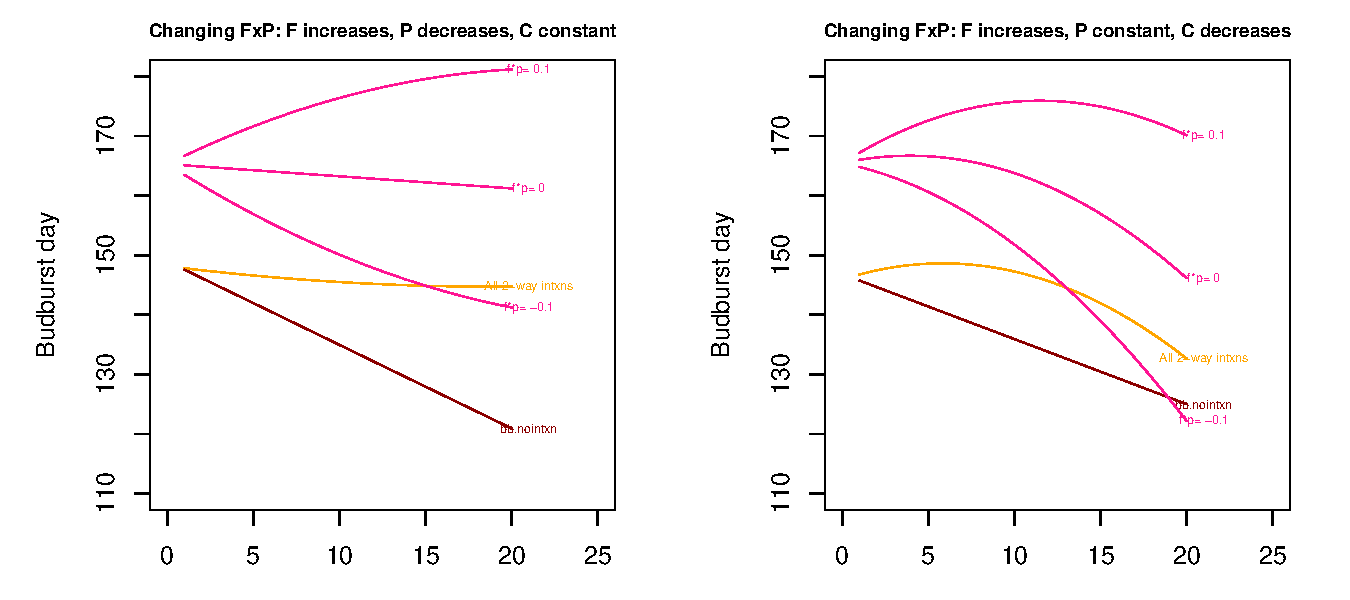
\includegraphics[width=1\textwidth]{..//..//analyses/limitingcues/figures/intxnsims_FPexample.pdf}
\caption{Interactions in linear models can produce nonlinearities \emph{if cues shift also} (and only if that, according to my work in nonlinearities\_intxns.R). Brown lines show a model of budburst without interactions, the yellow shows all two-way interactions and the pink lines vary the forcing x photoperiod interactions. In both cases we vary forcing, but on the left photoperiod decreases as forcing increases, while on the right chilling decreases while forcing increases.} % Dan writes: maybe a little more clear annotation— its hard to know whether a f*p of 0.1 or -0.1 is big.
  \label{fig:intxns}
\end{figure}
\clearpage



\begin{figure}[t!]
\centering
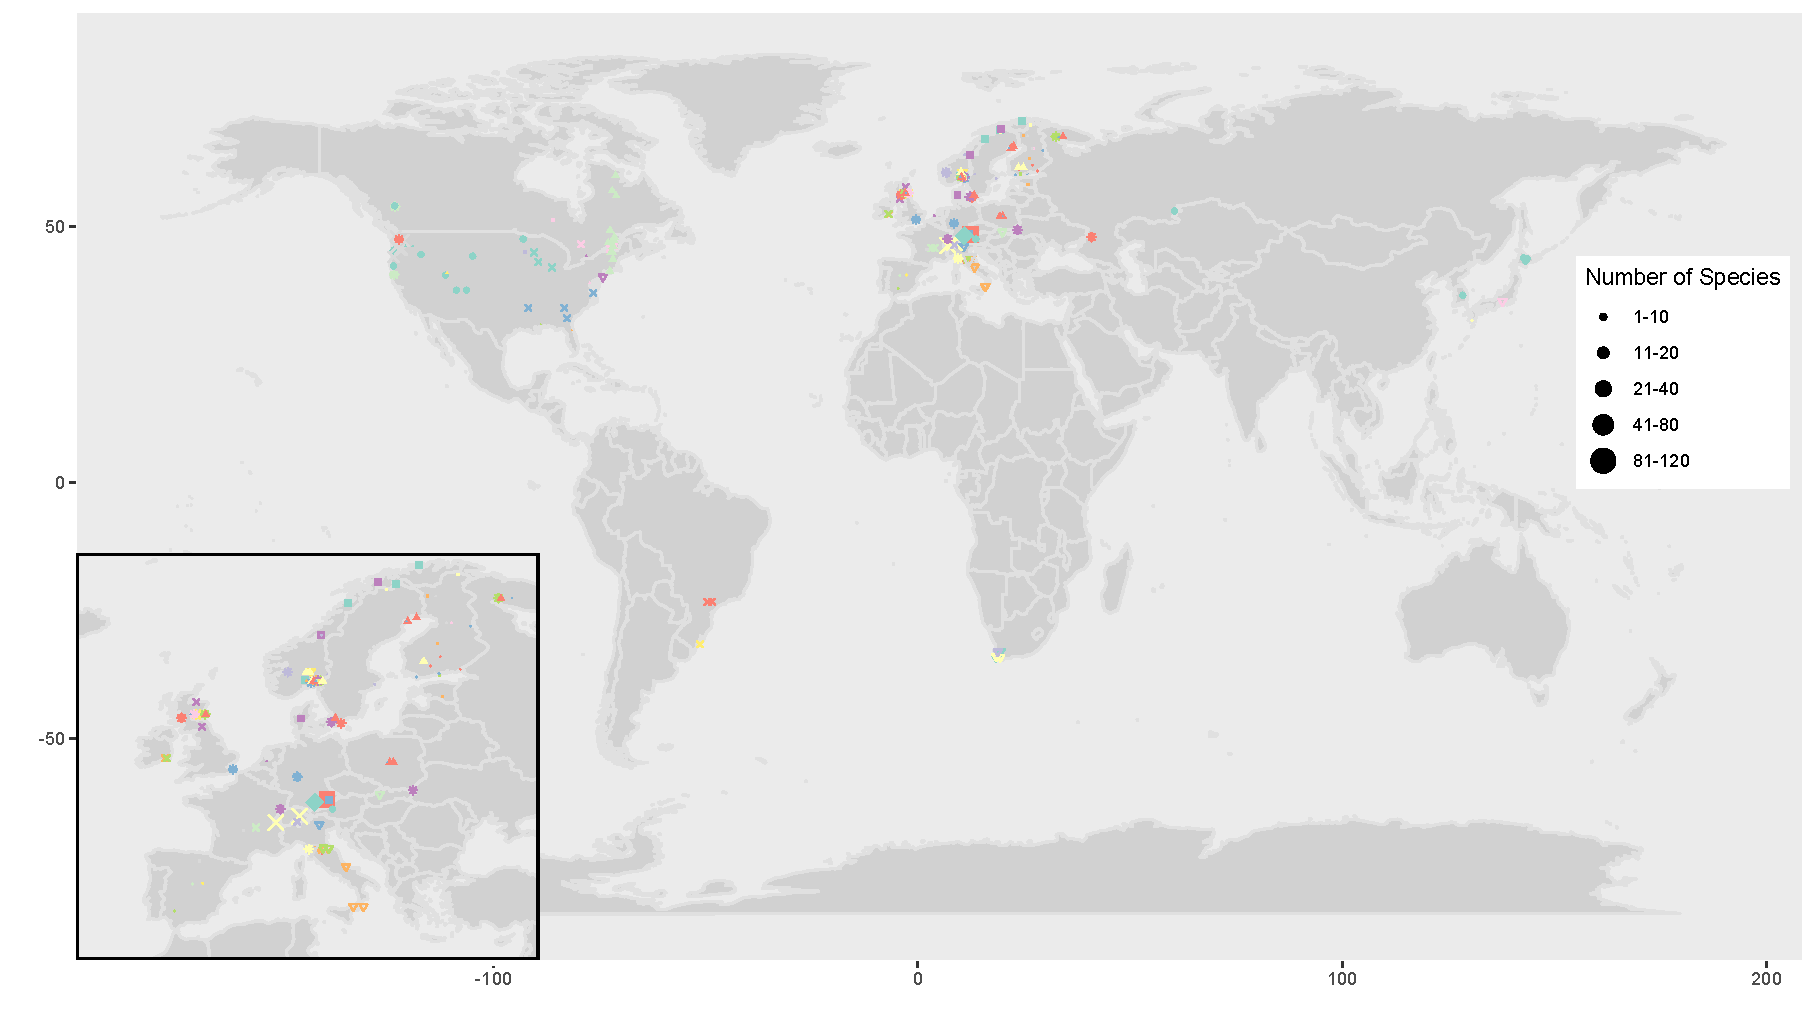
\includegraphics[width=1\textwidth]{..//..//analyses/limitingcues/figures/maps/map_studyspp.pdf}
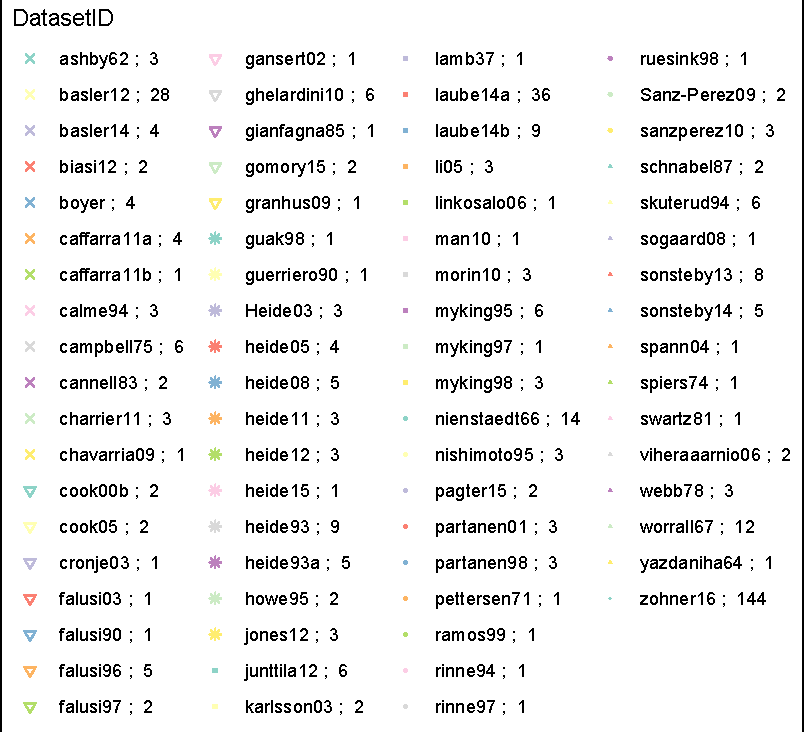
\includegraphics[width=0.5\textwidth]{..//..//analyses/limitingcues/figures/maps/map_studyspp_legend.pdf}
\caption{Overview of the data across space.}
  \label{fig:datamap} % Ailene: This figure is nice. i would say, though, that i don't find the size of the shapes to be particularly easy to interpret. seeing the numbers next to each study is a much more effective at showing that most studies have fewer than 5 spp.
\end{figure}
\clearpage


\begin{figure}[t!]
\centering
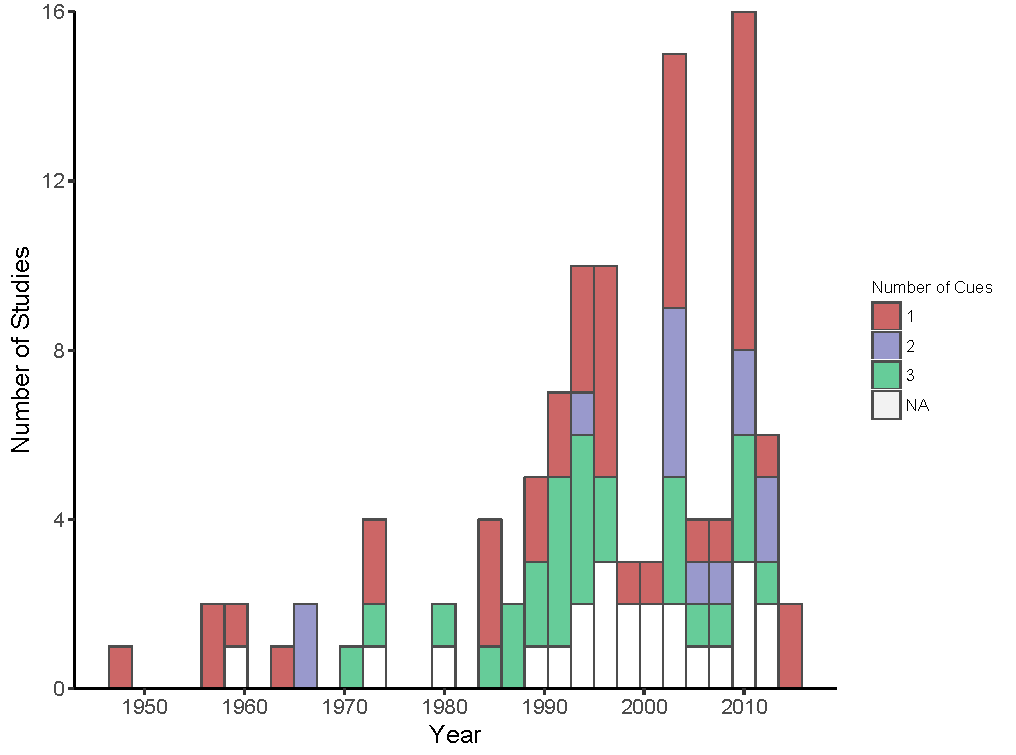
\includegraphics[width=1\textwidth]{..//..//analyses/limitingcues/figures/studyyearcues.pdf}
\caption{Cues manipulated over time.}
  \label{fig:ts}
\end{figure}
\clearpage

\begin{figure}[t!]
\centering
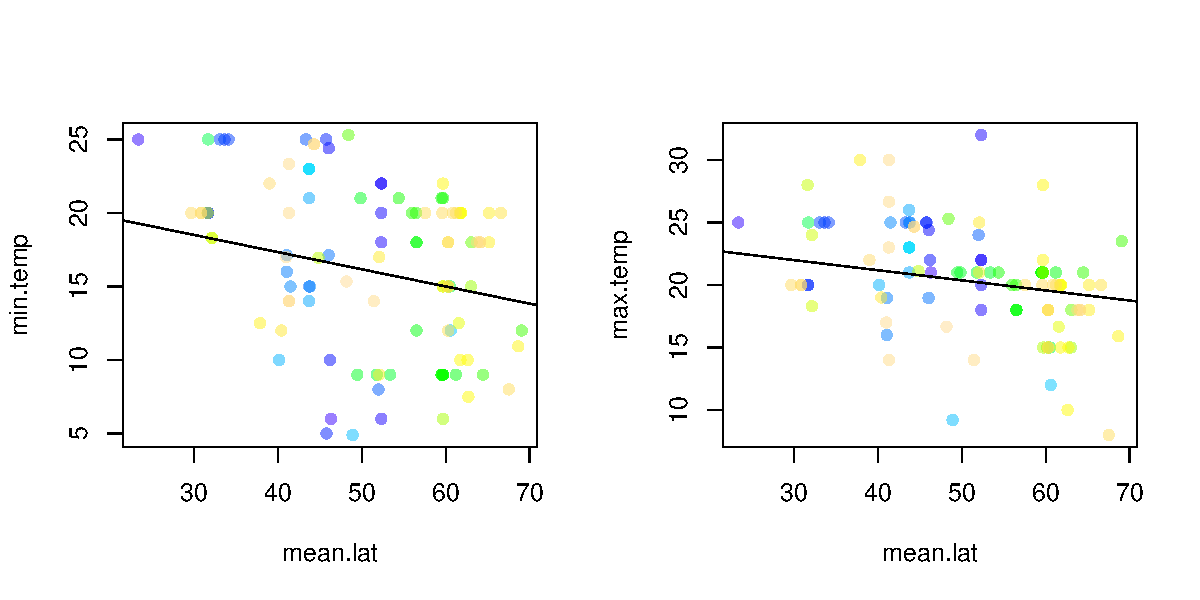
\includegraphics[width=1\textwidth]{..//..//analyses/limitingcues/figures/tempxlatminmaxcorr.pdf}
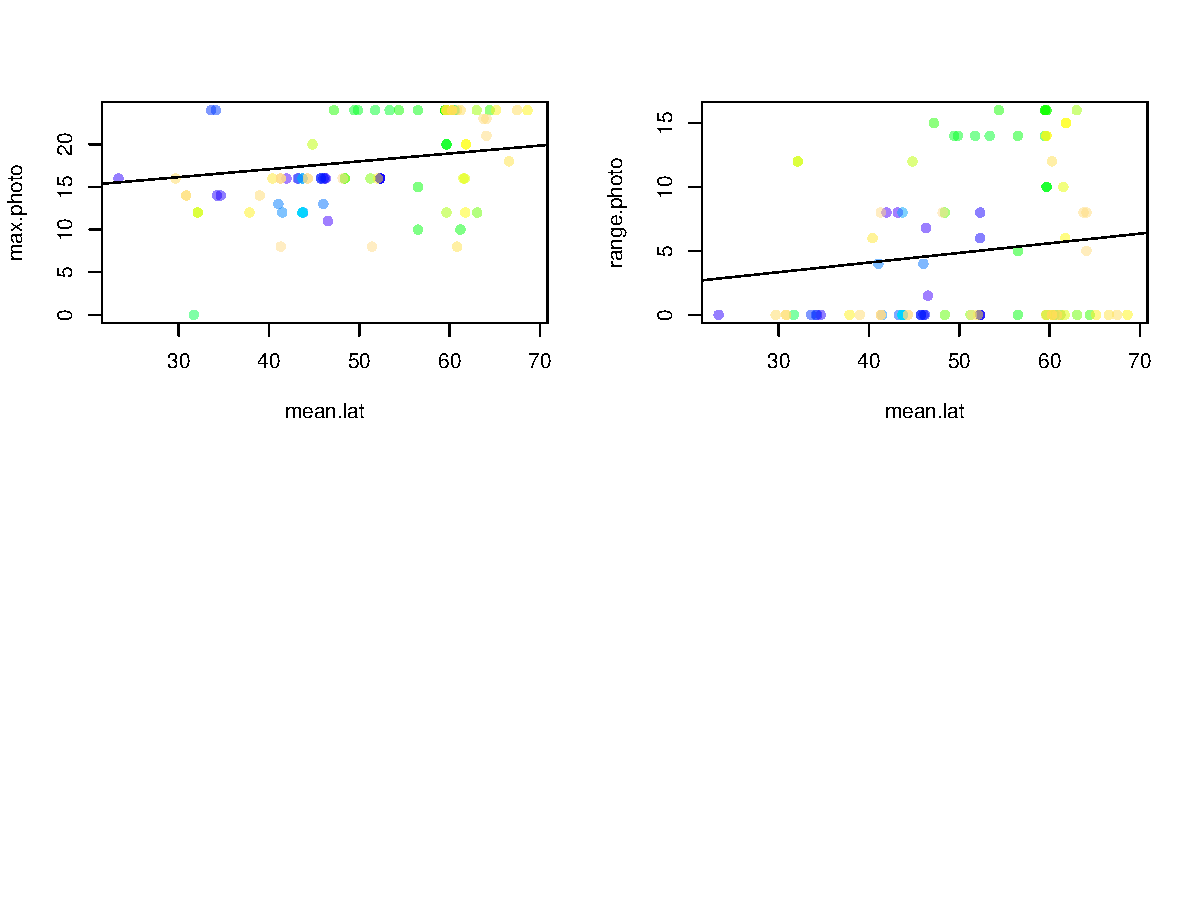
\includegraphics[width=1\textwidth]{..//..//analyses/limitingcues/figures/photoxlatcorr2plots.pdf}
\caption{One correlation with latitude plot? Or more?}
  \label{fig:lat}
\end{figure}
\clearpage



\begin{figure}[t!]
\centering
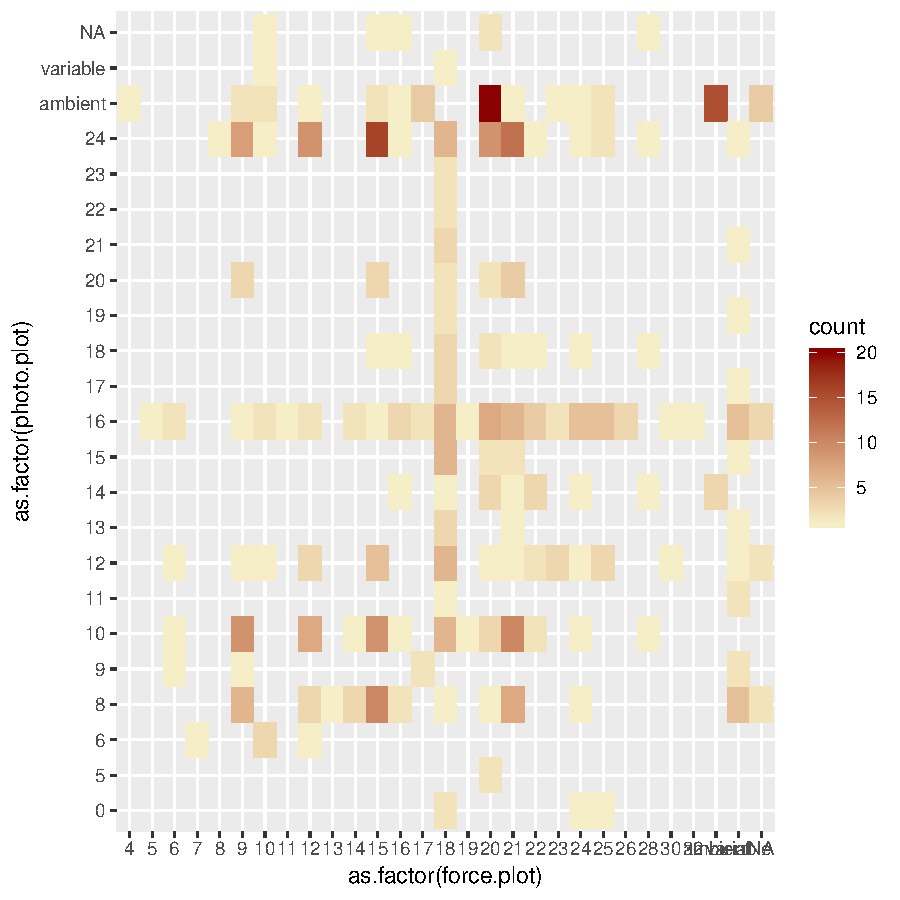
\includegraphics[width=0.3\textwidth]{..//..//analyses/limitingcues/figures/heatmapforcexphoto.pdf}
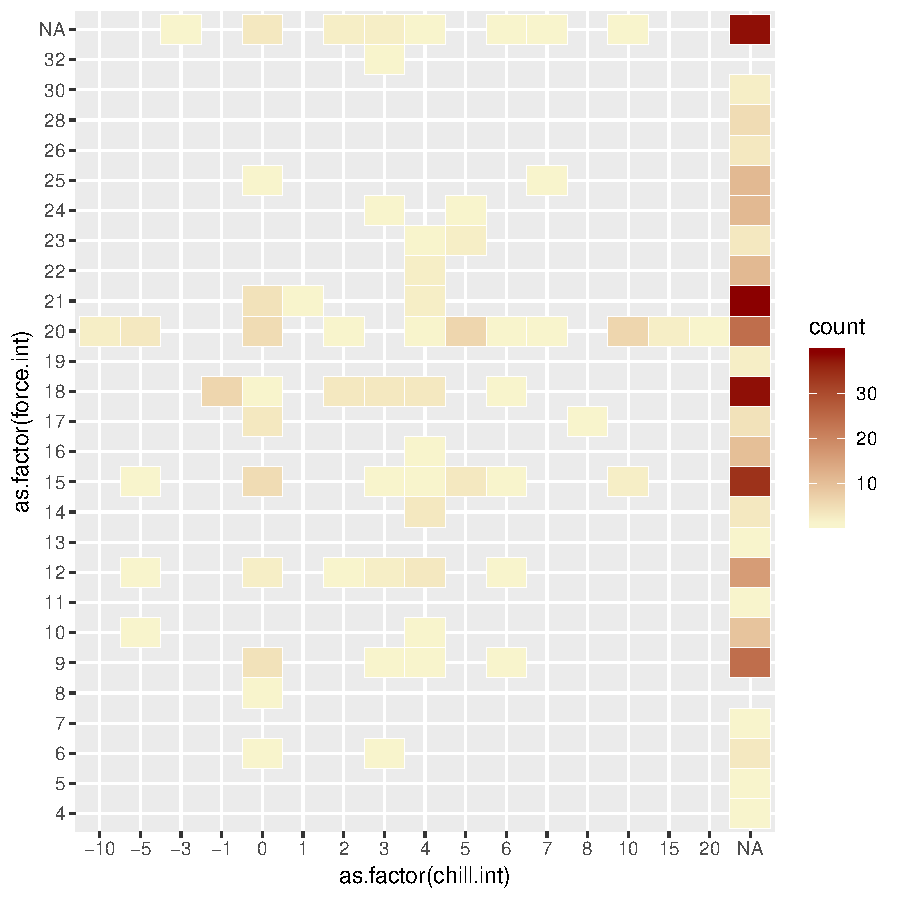
\includegraphics[width=0.3\textwidth]{..//..//analyses/limitingcues/figures/heatmapchillxforce.pdf}
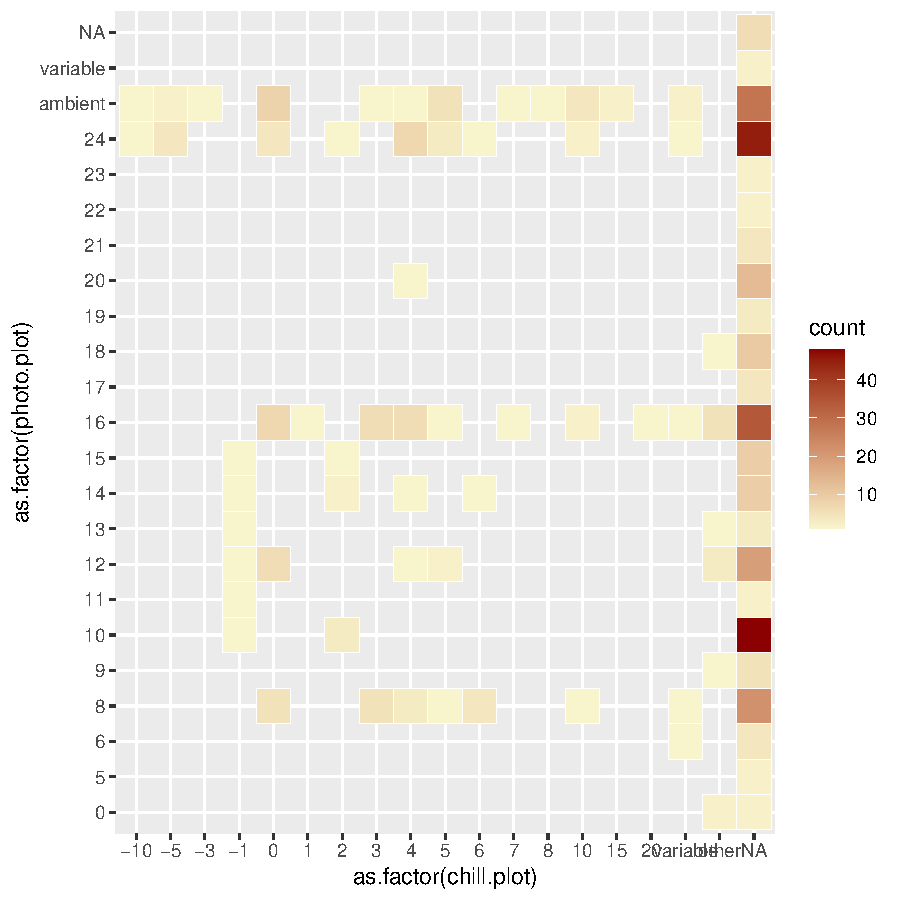
\includegraphics[width=0.3\textwidth]{..//..//analyses/limitingcues/figures/heatmapchillxphoto.pdf}
\caption{Our old heat maps, based only on what we could convert to numeric easily. See the next two figures please!}
  \label{fig:heatmaps} % Ailene: I find these heatmaps to be very overwhelming and hard to interpret. for example, there are so many NAs or 1s for field sample dates (are these studies that did not use the weinberger approach?) that I'm not sure what the take-home for readers should be- just that most studies use only 1 or no field sample dates?Similarly, for chilltemp vs photoperiod or forcing, is the main point that there are many unexplored combinations? if so, then i suppose this shoes that well and with cleaning up the nonnumeric values i think it could work.
\end{figure}
\clearpage


\begin{figure}[t!]
\centering
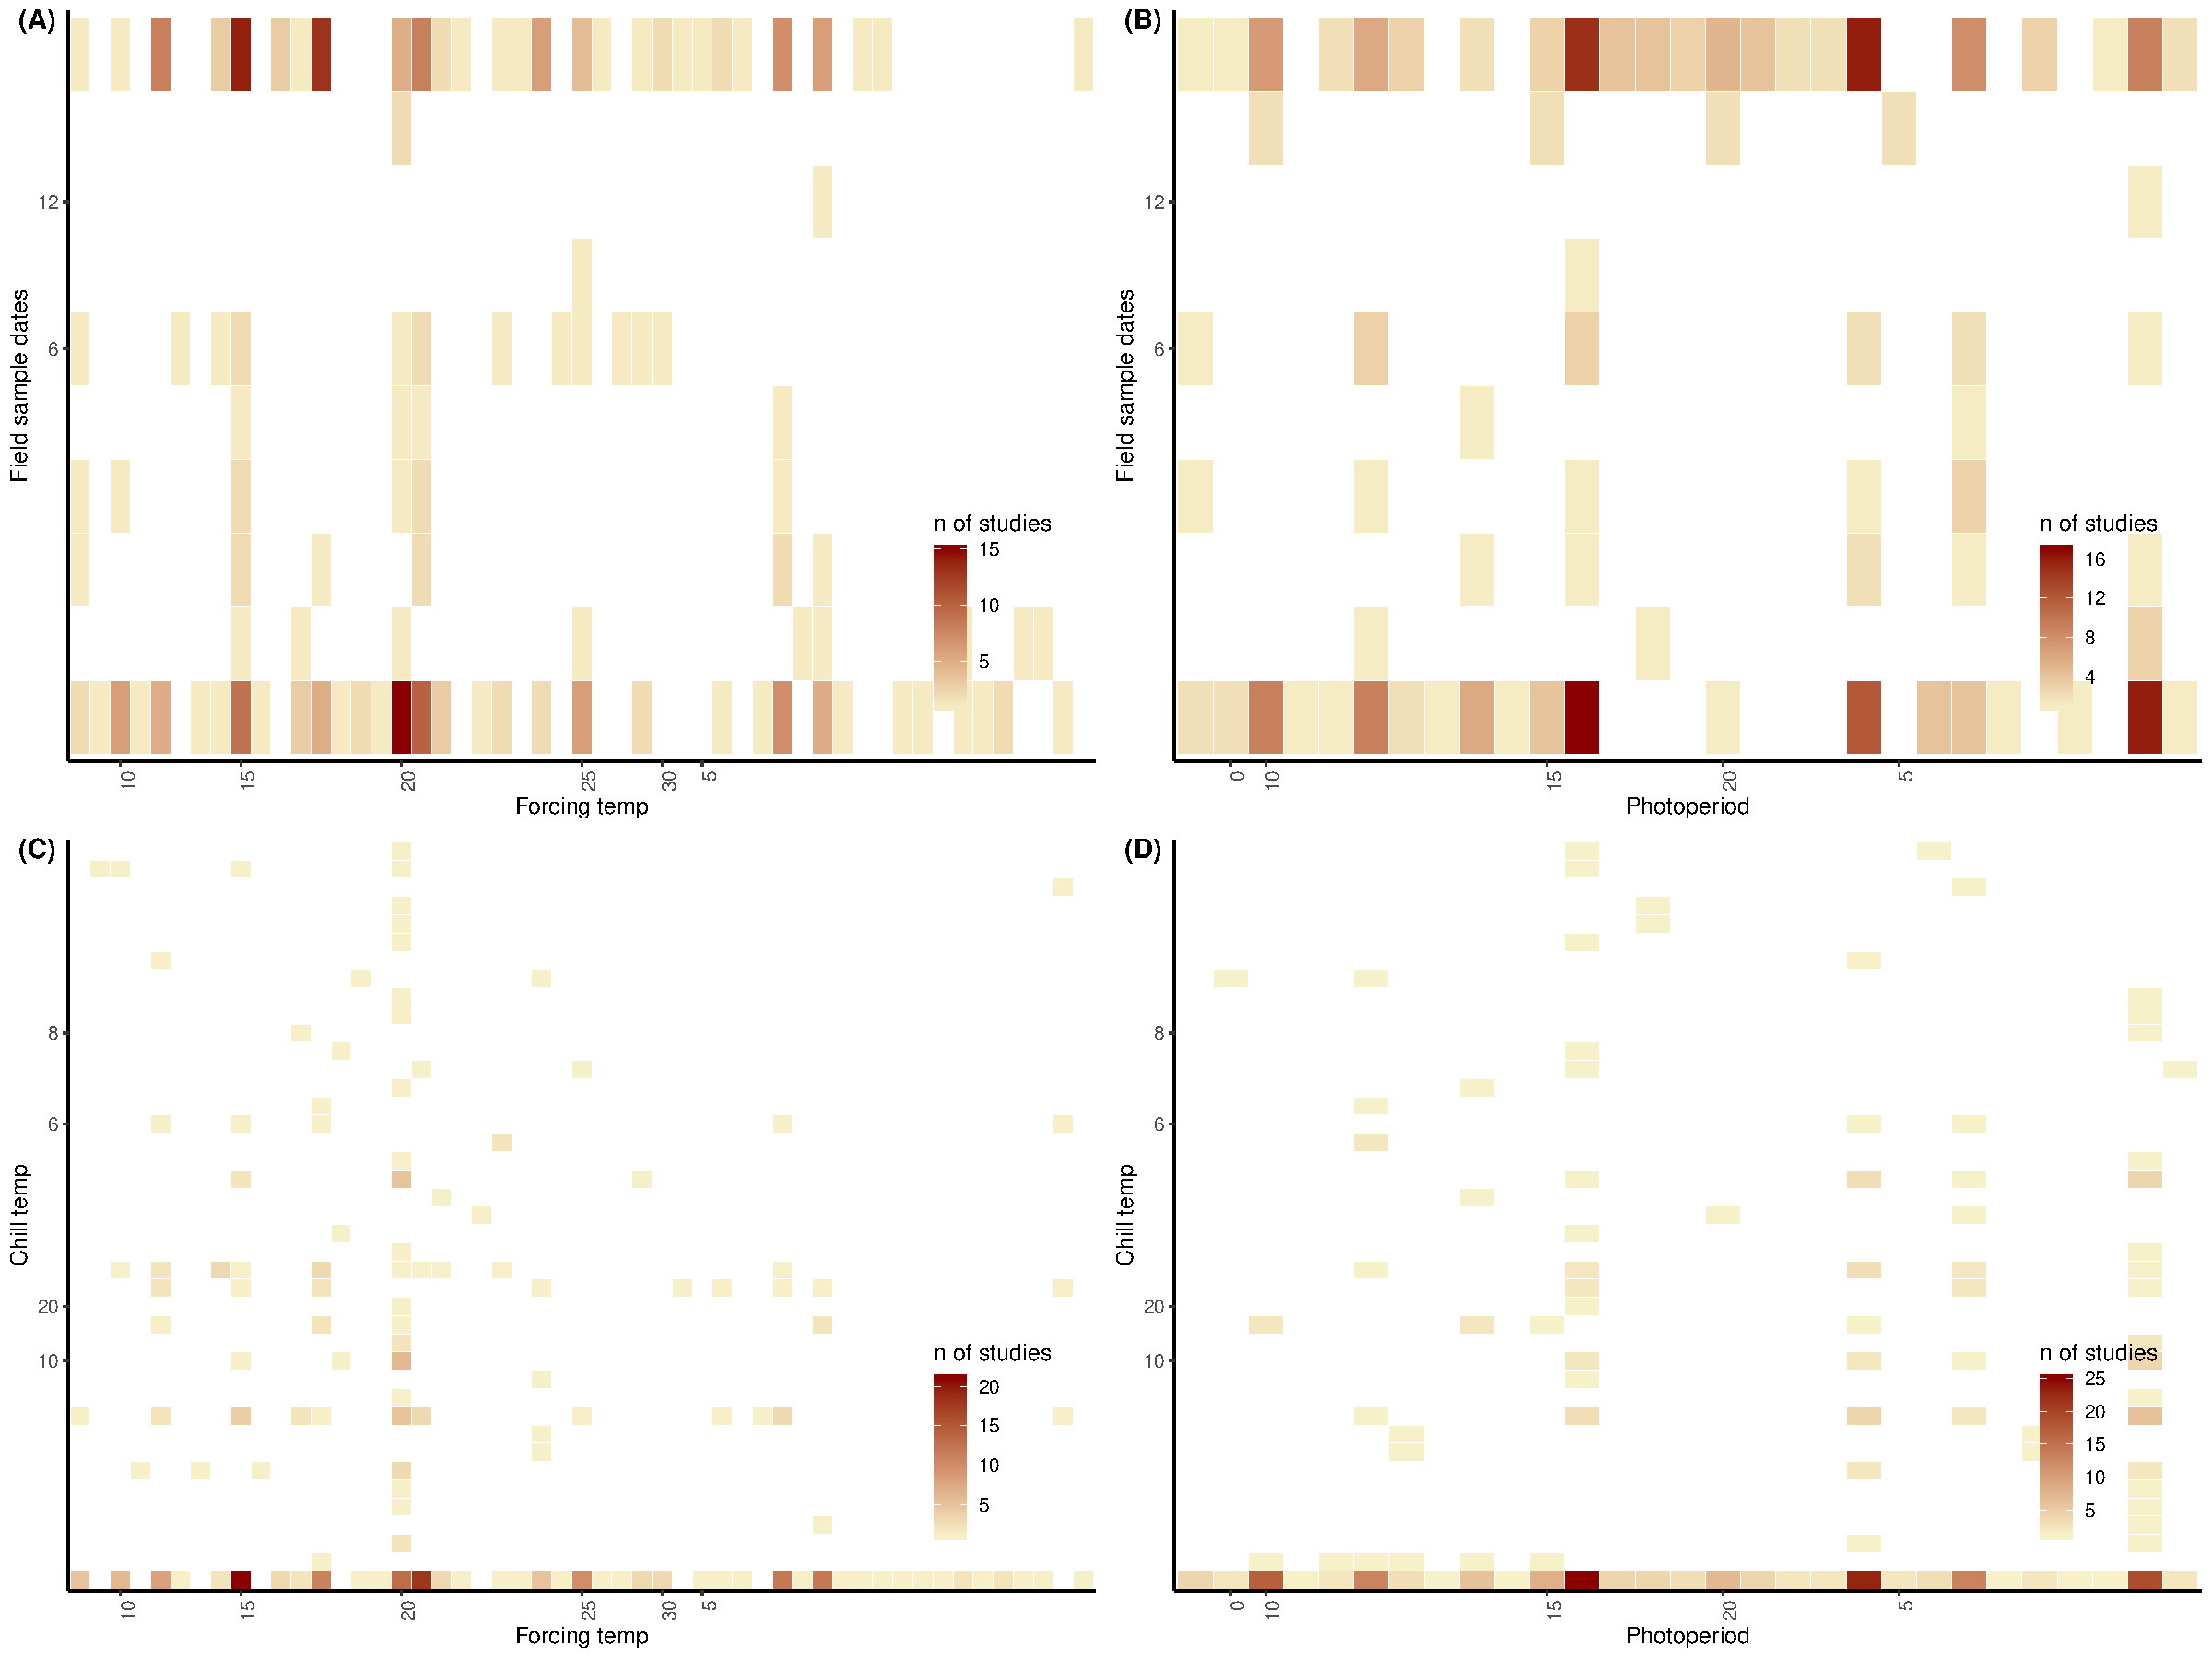
\includegraphics[width=1\textwidth]{..//..//analyses/limitingcues/figures/heatallosp_4panel.pdf}
\caption{Heatmap using all woody species data in OSPREE: shows number of studies for different study designs (we could clean this up in various ways ... perhaps only show budbreak or budburst studies?).}
  \label{fig:heatmap4p}
\end{figure}


\begin{figure}[t!]
\centering
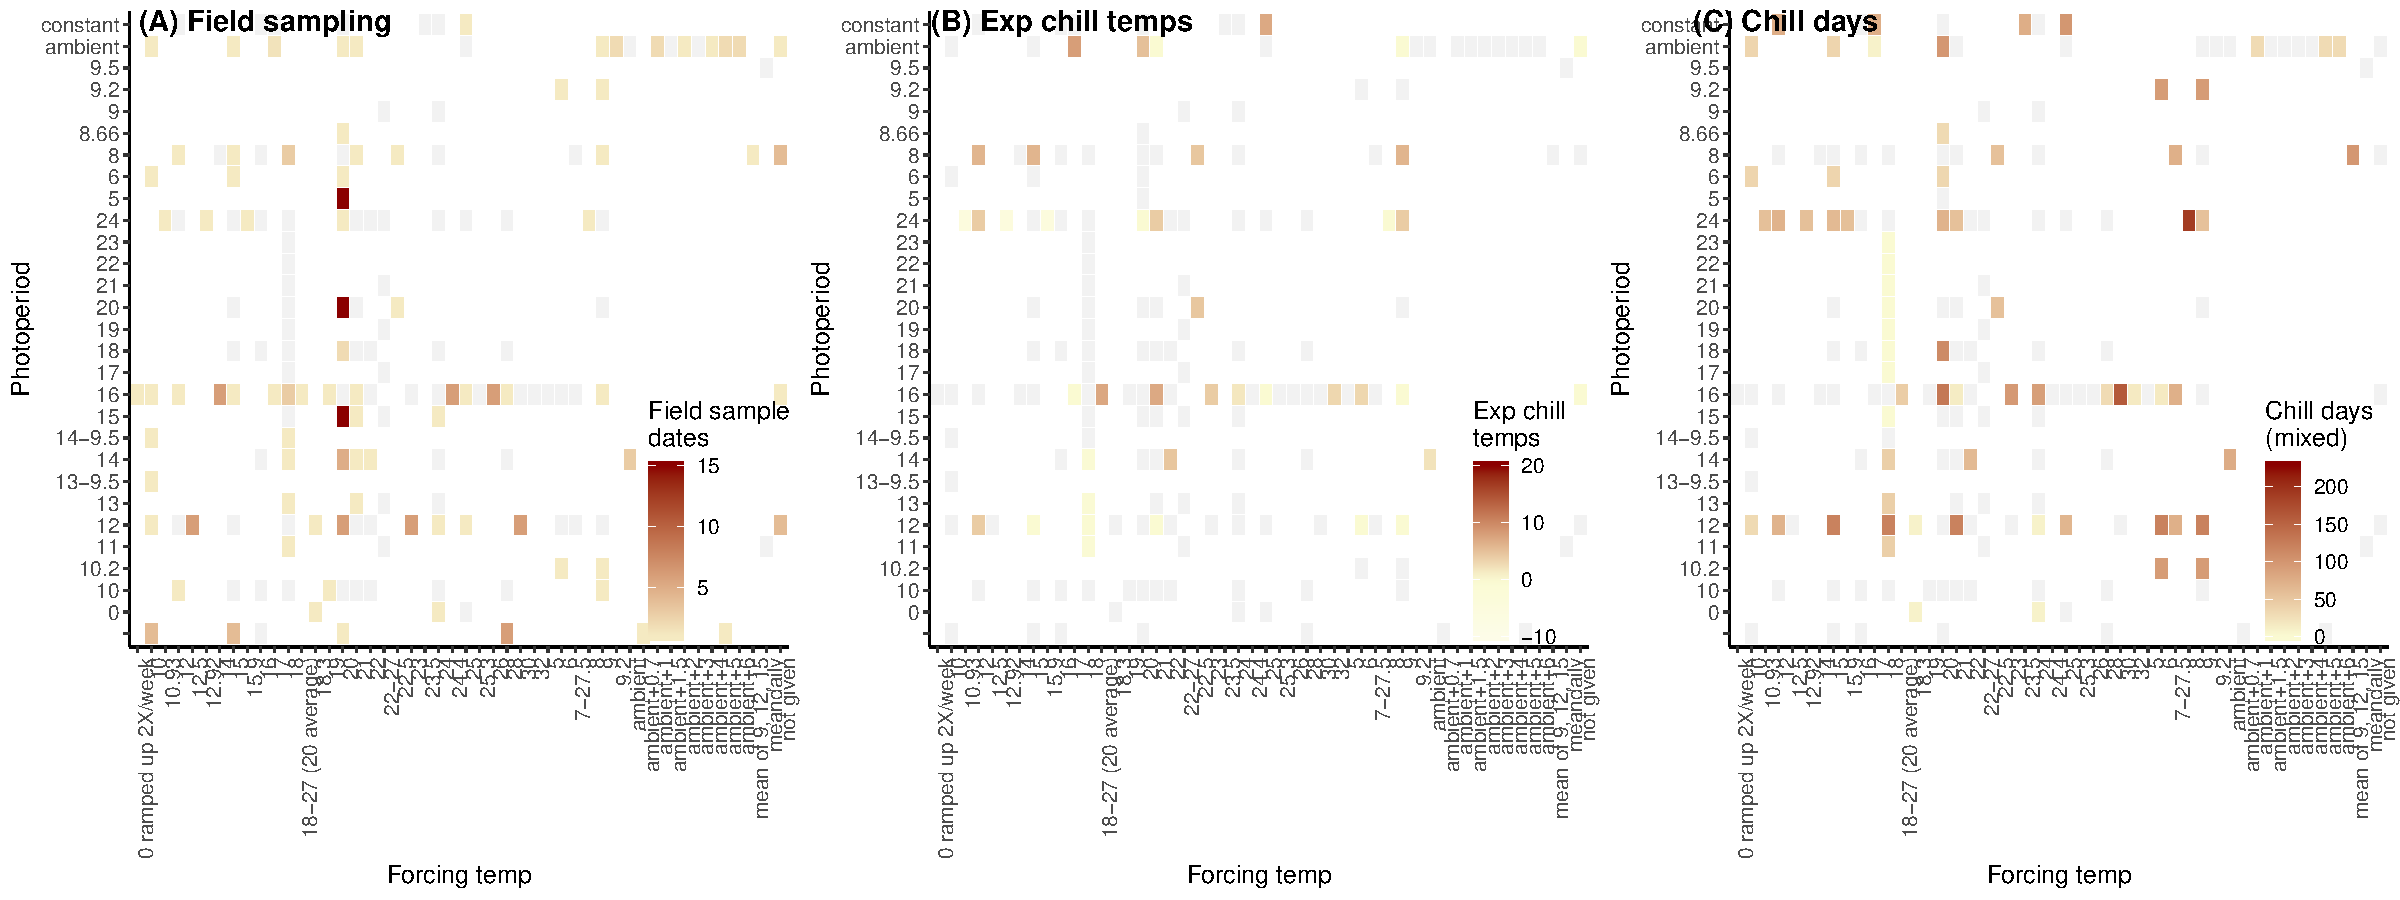
\includegraphics[width=1\textwidth]{..//..//analyses/limitingcues/figures/heatallosp_3treats.pdf}
\caption{Heatmap using all woody species data in OSPREE and attempting to show three-way treatments (note that chilldays includes a mix of experimental chilling and field-sample day chilling; this could be very tricky to clean up).}
  \label{fig:heatmap3p}
\end{figure}



\end{document}